\documentclass{article}
\usepackage[pdftex]{graphicx}

\title{Pythorient - a lightweight script to add some functionality in the analysis of EBSD data}

\author{J\"orn Leuthold}


\date{\today}
% Hint: \title{what ever}, \author{who care} and \date{when ever} could stand 
% before or after the \begin{document} command 
% BUT the \maketitle command MUST come AFTER the \begin{document} command! 
\begin{document}

\maketitle


\begin{abstract}
Pythorient is developed for the identification of CSL $\Sigma$ triple junction (TJ) configurations, which is particularly useful for the characterization of the microstructure in terms of grain boundary engineering. During recrystallization at elevated temperatures the migration of grain boundaries (GB) result in an increased probability of the formation of a $\Sigma3-\Sigma3-\Sigma3^n$ $(n \geq 2)$ TJ in low stacking fault metals. This special orientation relationship affects the properties of a material in terms of crystal plasticity, creep and corrosion resistance. Understanding the processes in the microstructure which lead to a inhomogeneous distribution of CSL TJs help to improve such macroscopic properties. 


\end{abstract}

\section{Brief overview of the program}
Pythorient reads HexGrid files exported from OIM Analysis (vers. 5.3). Cleaning procedures have to be done in advance. Depending on the overall quality of the EBSD measurement, a dilation cleaning -though dangerous in term of creation of artifacts- is recommended in order to remove non-indexed points. Also the rain-fall segmentation to extract the grain partition has to be carried out in OIM Analysis (which is done by default). By default the data file contains:   phi1, Phi, phi2, x, y, IQ, CI, Fit, ID, edge, phase. The Euler angles must be given in rad (not deg). General GBs and TJs are determined from Grain ID. CSL GBs and TJs are computed with respect to the crystal symmetry and point group (so far only Cubic and fcc). For plotting either a common map (so far IPF, IQ) or density estimation map of a given TJ configuration is created. The density estimation can be undertaken by a boxsum or gaussian method.
\begin{figure}[ht]
\centering
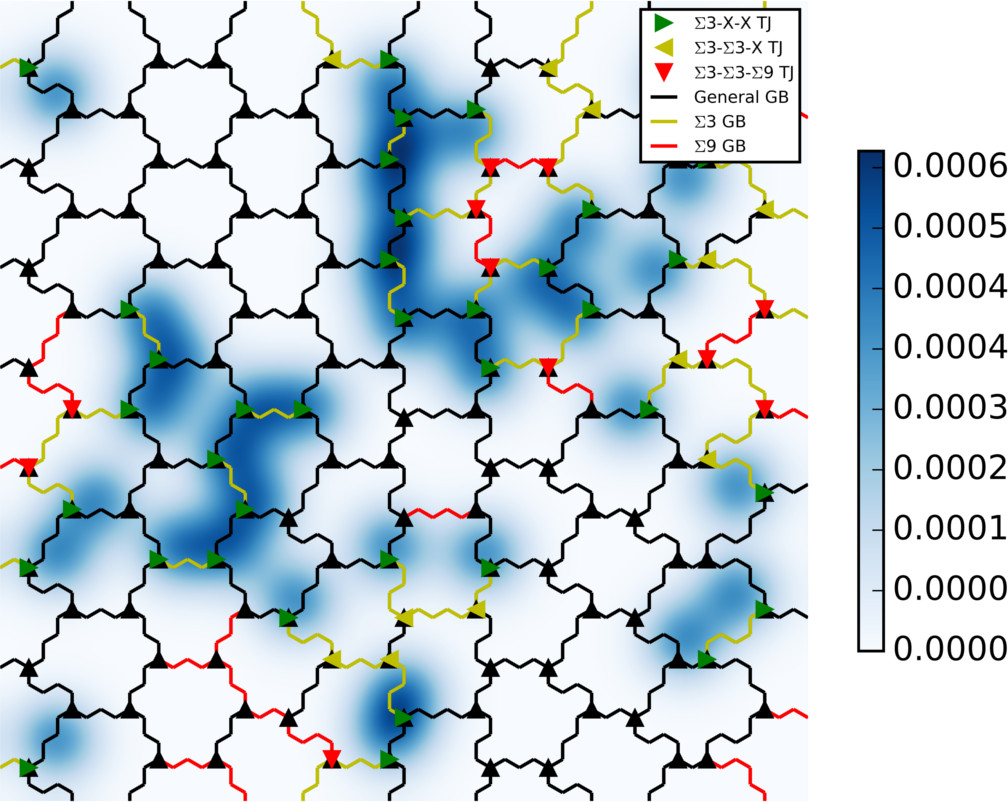
\includegraphics[width=\linewidth]{figs/Generated_OIM}
\caption{Example of TJ analysis on a artificially generated microstructure. For density estimation only $\Sigma3-X-X$ TJs are taken into account.}
\label{fig:generated}
\end{figure}

\begin{figure}[ht]
\centering
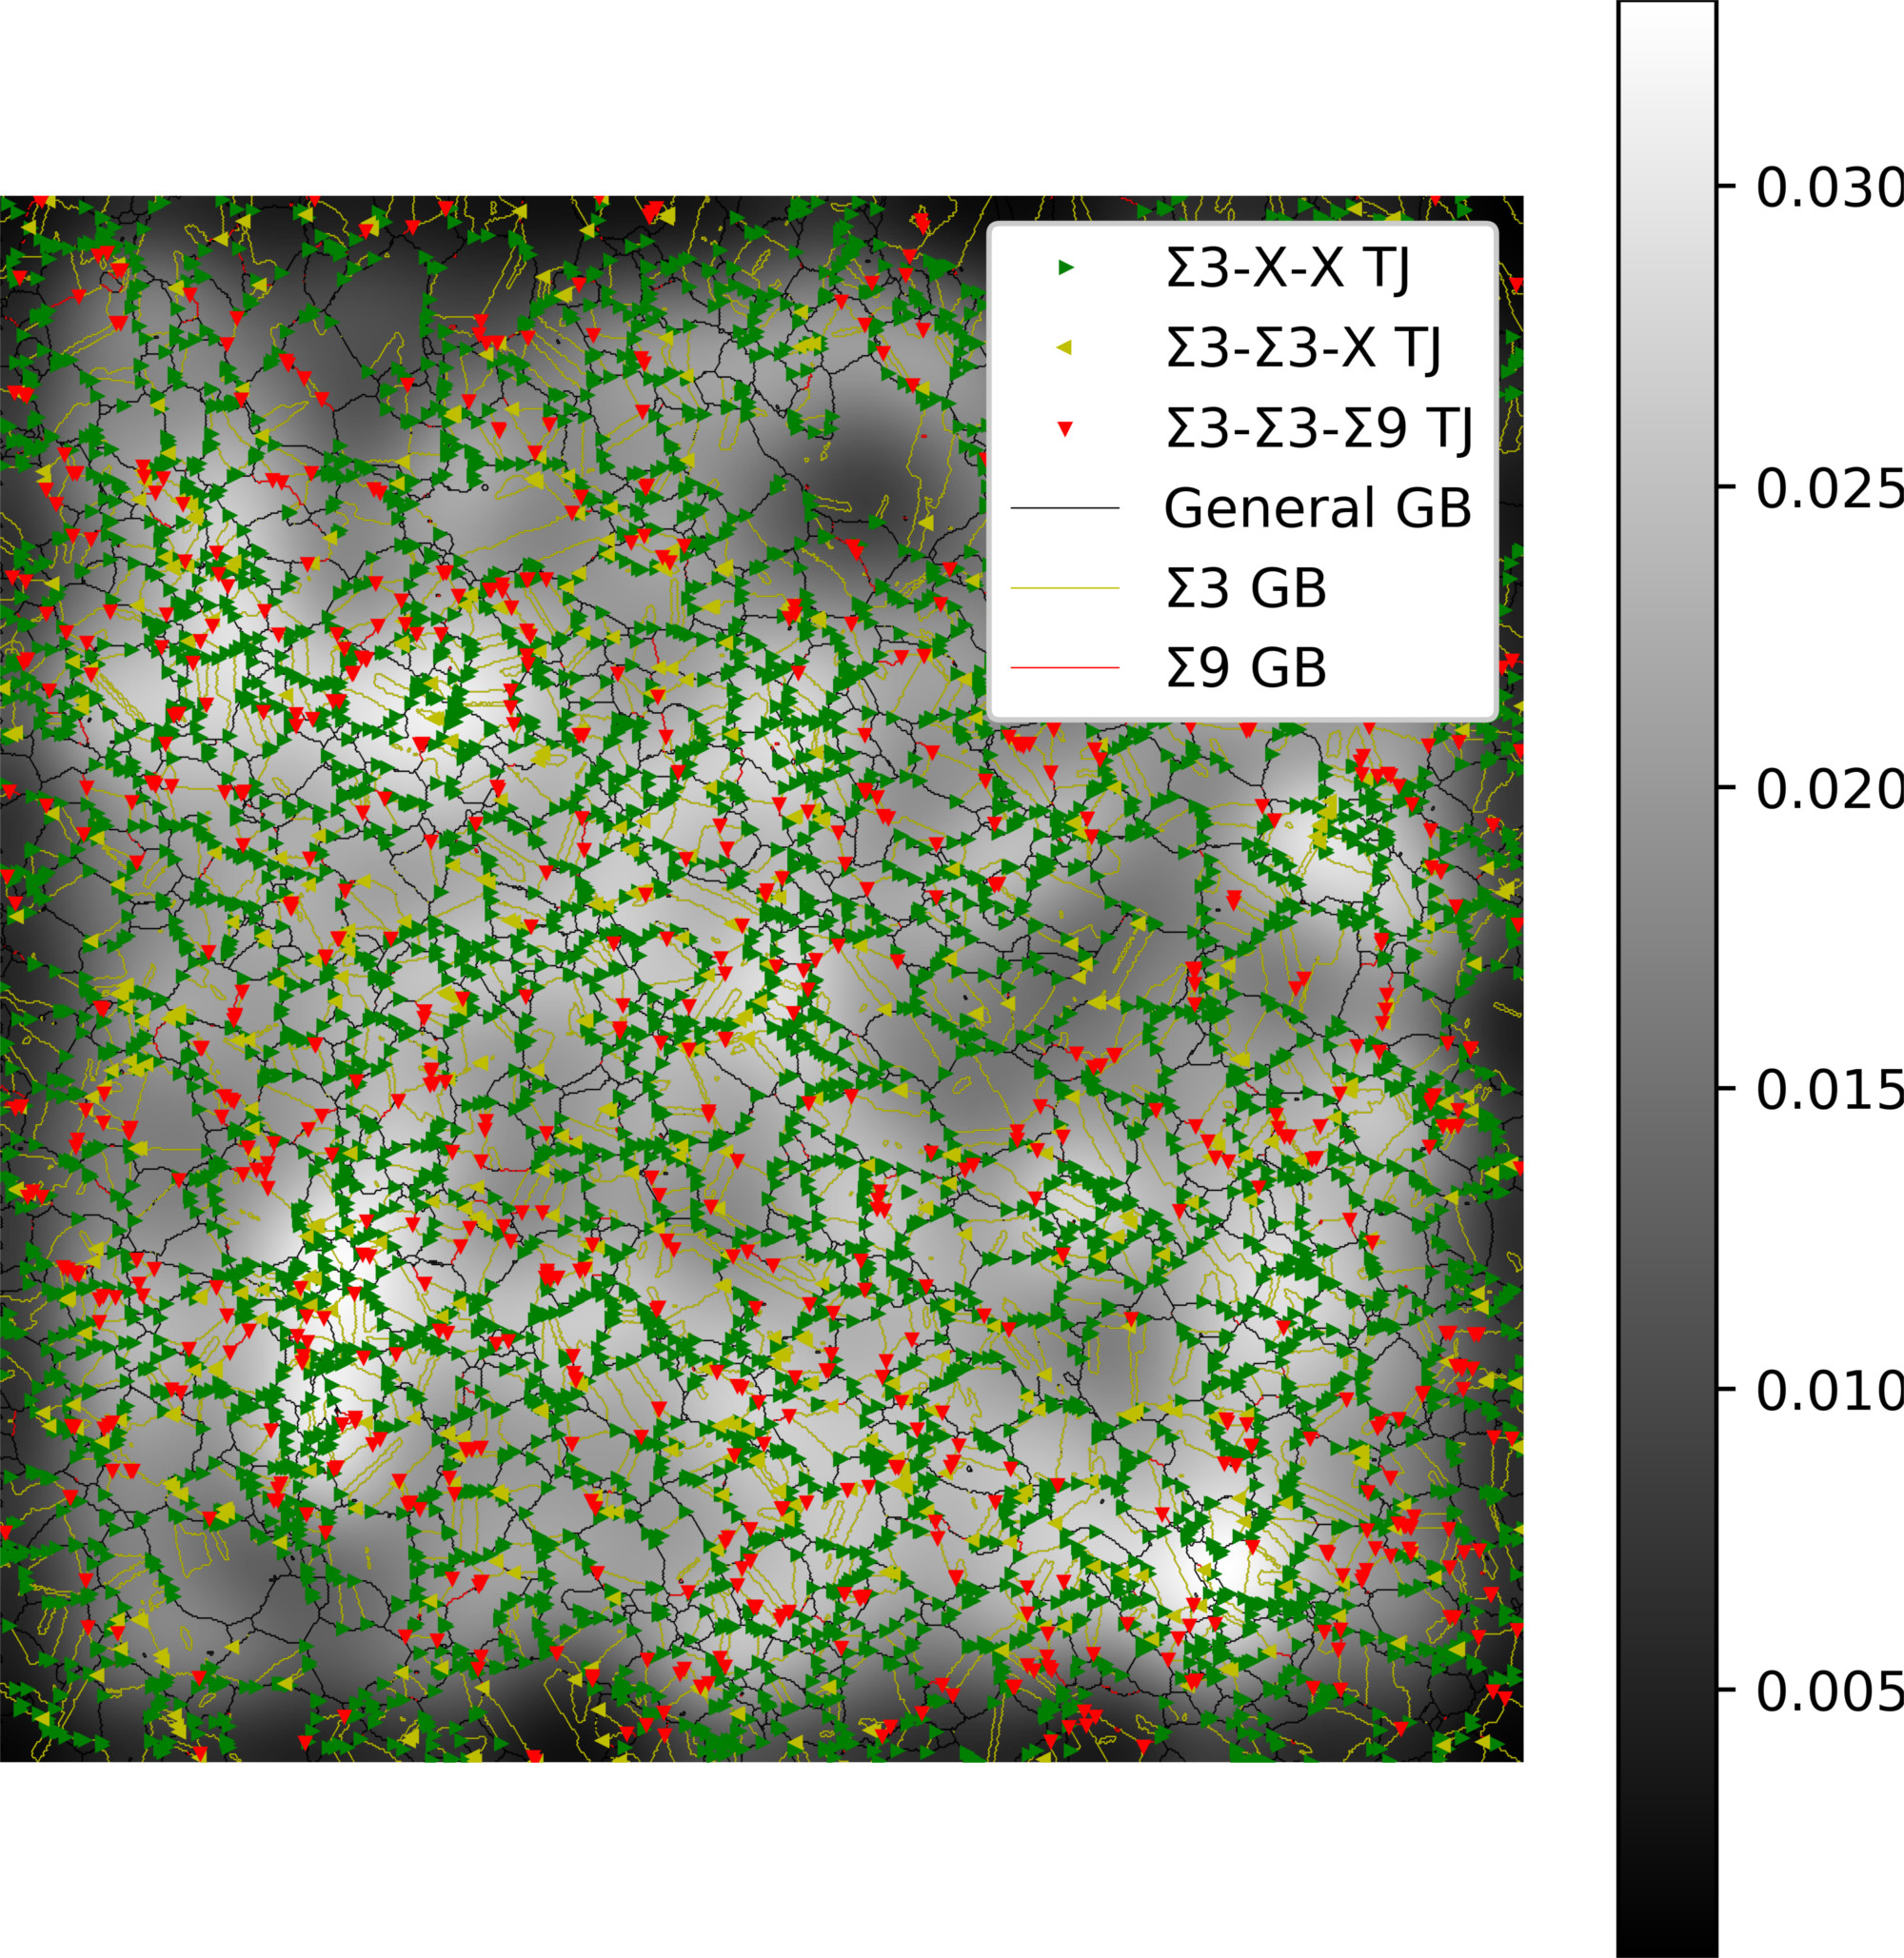
\includegraphics[width=\linewidth]{figs/Cu_TJ_analysis}
\caption{TJ analysis on a Cu sample subjected to annealing after severe plastic deformation.}
\label{fig:Cu_SPD}
\end{figure}
\end{document}

